\section{Schéma simplifié du cycle de vie d'un projet}
\newImageAnnexe[H]{0.75}{cycle-vie-projet.png}{cycleVieProjet}

\clearpage
\section{Construction des modules communs de l'application au sein d'un projet \naq}
\newImageAnnexe{0.9}{modules.png}{commons-modules}

\clearpage
\section{Build continu d'un projet \naq}
\begin{figure}[ht]
	\centering
	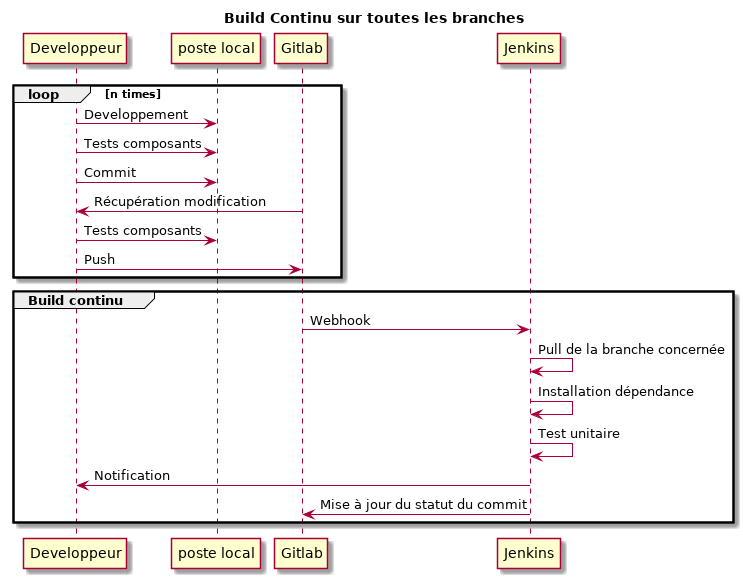
\includegraphics[scale=0.6,angle=-90]{img/build-continu.png}
	\label{annexe:build-continu}
\end{figure}

\clearpage
\section{Flux de travail du déploiement d'une version d'un site \naq}
\newImageAnnexe{0.32}{release.png}{release-naq}

\clearpage
\section{Matrice de développement \devops}

\normalsize{Source : \url{https://www.infoq.com}}

\begin{figure}[ht]
	\centering
	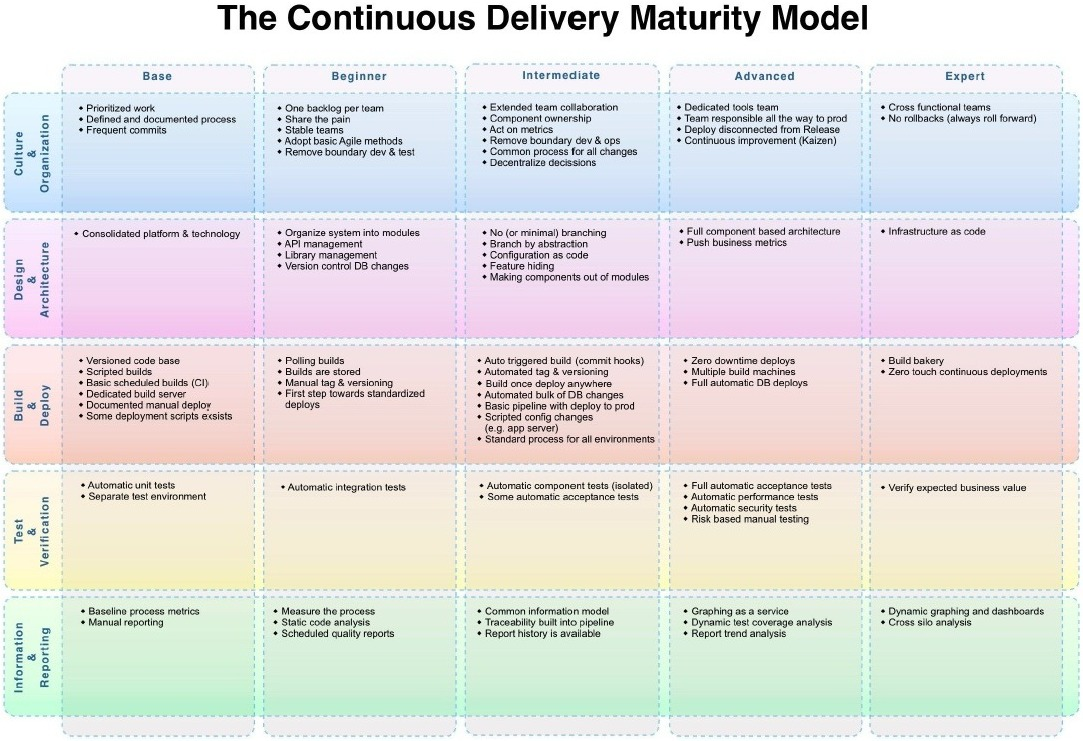
\includegraphics[scale=0.62,angle=-90]{img/devops-matrice.jpg}
	\label{annexe:devops-matrice}
\end{figure}

%\clearpage
%\section{Flux de travail pour un hotfix sur un site \naq}
%\newImageAnnexe{0.25}{hotfix.png}{hotfix-naq}